\subsection{Desarrollo de la idea.}

\vspace*{0.3cm}

Sea $G$ un grafo cualquiera, $I$ un conjunto independiente de ese nodo, y $n_{1}$,$n_{2}$ nodos de G que no pertenecen a $I$ y no tienen aristas en común con ningún elemento de $I$, diremos que $n_{1}$ es óptimo si no existe ningún $n_{2}$ tal que $( \# (Vecinos(n_{2})) - \# (Vecinos(n_{2}) \cap Vecinos(I))) > ( \# (Vecinos(n_{1})) - \# (Vecinos(n_{1}) \cap Vecinos(I)))$. Definimos $Vecinos(\alpha)$ como el conjunto de nodos a los cuales $\alpha$ lleva una arista si $\alpha$ es un nodo, y si $\alpha$ es un conjunto, entonces es el conjunto de nodos a los cuales les llega un arista desde por lo menos un elemento de $\alpha$.  De manera más informal, podemos decir que un nodo óptimo es aquél que más vecinos ``libres'' tiene, siendo un nodo ``libre'' uno que no está en el conjunto solución ni es adyacente a un nodo de la solución.

Nuestra heurística se basa en formar un conjunto independiente maximal de la siguiente manera:
Primero, considerando al conjunto independiente vacío, tomamos a un nodo óptimo, y lo agregamos como nuevo elemento de nuestro conjunto independiente. Luego con nuestro nuevo conjunto independiente, tomamos un nodo óptimo, y lo agregamos a nuestro conjunto independiente. Repetimos esto hasta que no exista un nodo óptimo, puesto que nuestro conjunto independiente se transformó en maximal, y por lo tanto en un conjunto dominante.
 
\vspace*{0.6cm}

%\newpage

\subsection{Análisis de complejidad.}

\vspace*{0.3cm}

Pasemos a analizar la complejidad del algoritmo en cuestión, tal vez abstrayendonos del peor caso, pero si tratando de maximizar los costos de los distintos pasos a realizar. Notemos primero que buscar el nodo ``óptimo'' nos toma $\mathcal{O}(n)$ ya que se trata de recorrer los nodos del grafo haciendo comparaciones sobre la cantidad de vecinos que possen $\mathcal{O}(1)$. (Creo que no sería errado decir que si entro $n$ veces a buscar al optimo, es porque todos tenian grado 0, sino se irian eliminando posibilidades, por ende la complejidad seria $\mathcal{O}(n^2)$).


Supongamos un caso en el que debo entrar $n-1$ veces a buscar el ``óptimo'' $\mathcal{O}(n)$. Luego tendría un costo de $\mathcal{O}(n^2)$.


A este se le suma el costo de marcar a los nodos elegidos y a sus vecinos como ``tomados''. Para esto debemos tener en cuenta que marcarlos toma $\mathcal{O}(1)$, y que cada nodo puede tener como máximo $n-1$ vecinos, pero la suma total de nodos vecinos a marcar como tomados es siempre $n-1$ ($\mathcal{O}(n)$). Luego, y ya metiéndonos un poco con lo que respecta a la implementación, debemos actualizar los grados de los nodos vecinos de los vecinos del nodo tomado como ``óptimo''. Como ya dijimos, la suma de los vecinos del nodo tomado puede llegar a $n-1$, y estos a su vez podrían llegar a tener $n-1$ vecinos. Como debo recorrerlos para actualizarlos estaríamos hablando de una complejidad de $\mathcal{O}(n^2)$


Por último la solución del algoritmo consiste integrar cada nodo ``óptimo'' a la solución final, lo que puede llegar a tomar $\mathcal{O}(n)$.

Siendo $T(n)$ la complejidad de nuestro algoritmo tenemos:

\begin{equation*}
\begin{array}{l}
T(n) = \mathcal{O}(n^2) + \mathcal{O}(n) + \mathcal{O}(n^2)\\
T(n) = 2\mathcal{O}(n^2)
T(n) = \mathcal{O}(n^2)
\end{array}
\end{equation*}

\begin{figure}
\begin{codebox}
\Procname{$\proc{CIDM_goloso}(lista\_nodos$ $cidm\_sol)$} 
\li $res \leftarrow$ 0
\li \While no se hayan ``tomado'' todos los nodos
\li 	\Do 
 		$elegido \leftarrow$ nodo ``óptimo''
\li 		$cidm\_sol \leftarrow$ agregar $elegido$
\li 		incrementar $res$
\li 		marcar a $elegido$ y a sus vecinos como ``tomados''
	\End
\li \Return $res$
\end{codebox}
\caption{Heurística golosa constructiva para CIDM}\label{code:goloso}
\end{figure}
%\FloatBarrier

\vspace*{0.6cm}
%\newpage

\subsection{Instancias no óptimas.}

\vspace*{0.3cm}

A continuación presentaremos dos familias de grafos para las cuales nuestra heurística golosa no siempre encuentra una solución óptima.

\subsubsection*{Familia 1 - Estrellas}

La forma de los grafos pertenecientes a esta familia responde a las siguientes características:

\begin{itemize}
\item Existe un único vértice $v$ con grado máximo.  Sea $\delta_{max}$ el grado de este nodo.
\item Para cada vértice $w$ adyacente a $v$, $\delta(w) < \delta_{max}$, y sus nodos adyacentes (salvo $v$) tienen grado 1.	
\end{itemize}

Dado que el algoritmo propuesto va tomando en cada paso el nodo ``óptimo'', o sea, aquél que más nodos ``libres'' cubre, en un grafo como el descrito primero tomará al vértice $v$ con grado máximo $\delta_{max}$.  Luego, para cumplir con la independencia y la dominancia, deberá tomar a los vértices adyacentes a los vecinos de $v$. Como el grado de cada vecino de $v$ es menor a $\delta_{max}$, el peor de los casos sería que cada uno de ellos tuviera grado $\delta_{max} - 1$.  En este caso, cada vértice adyacente a $v$ tendría $\delta_{max} - 2$ vecinos además del mismo $v$, y entonces la solución hallada por nuestra heurística estaría conformada por $\delta_{max} \times (\delta_{max} - 2)$ nodos.  Sin embargo, para un grafo como el detallado, existe una solución mejor conformada por $\delta_{max}$ nodos, y corresponde al conjunto compuesto por los vecinos del nodo $v$.

La Figura \ref{fig:familia1} muestra un ejemplo de grafo perteneciente a esta familia, y la Figura \ref{fig:familia1res} muestra en color verde la solución hallada por nuestro algoritmo, la cual claramente es peor que la solución formada por los vértices que quedaron en rojo en la misma Figura.

\begin{figure}[!htb]
\minipage{0.5\textwidth}
\begin{center}
  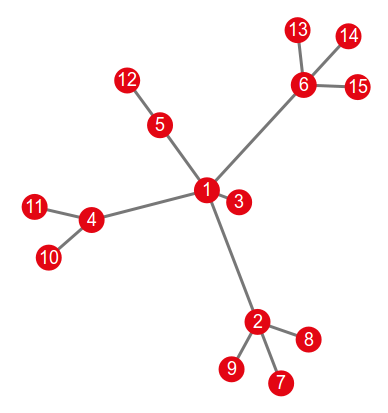
\includegraphics[scale=0.5]{imagenes/familia1.png}
\end{center}
  \caption{Grafo perteneciente a la Familia 1}\label{fig:familia1}
\endminipage\hfill
\minipage{0.5\textwidth}
\begin{center}
  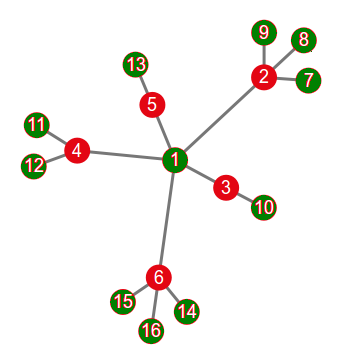
\includegraphics[scale=0.5]{imagenes/familia1-res.png}
\end{center}
  \caption{Solución hallada por nuestra heurística}\label{fig:familia1res}
\endminipage
\end{figure}

\subsubsection*{Familia 2 - Circuitos}

Como miembros de esta familia consideraremos a los circuitos simples.  Para este tipo de grafos, la calidad de la solución hallada por nuestro algoritmo dependerá de la cantidad de vértices que tenga y de la forma en que se hayan rotulado los mismos.

Consideremos un circuito $C_{n}$ y supongamos por un momento que los vértices están rotulados como $v_1,v_2,...,v_n$ tal que existe una arista entre $v_i$ y $v_j$ cuando $j = (i+1) mod (n)$.

Una forma de armar un CIDM $C$ para este grafo podría ser la siguiente: [HABRIA QUE PROBARLO]

\begin{itemize}
\item Si $n \equiv 0 (3)$, tomar $C = \{v_i | i \equiv 1 (3)\}$.
\item Si $n \equiv 1 (3)$, tomar $C = \{v_i | 1 \leq i < n, i \equiv 1 (3)\} \cup \{v_{n-1}\}$.
\item Si $n \equiv 2 (3)$, tomar $C = \{v_i | 1 \leq i < n-1, i \equiv 1 (3)\} \cup \{v_{n-2}\}$.
\end{itemize}

Si el grafo está rotulado de esta forma, nuestro algoritmo procederá de la siguiente manera:

\begin{itemize}
\item El primer nodo ``óptimo'' hallado será $v_1$, así que lo incluirá en la solución y lo marcará como ``tomado'' junto a $v_2$ y $v_n$. Por lo tanto, $v_3$ y $v_{n-1}$ pasarán a poder cubrir 1 nodo ``libre'' cada uno, de existir éste (notar que para $n = 3$ todos los nodos ya quedan ``tomados'', y para $n = 4, v_3 = v_{n-1}$ y es el único nodo que queda ``libre'').
\item Mientras queden nodos ``libres'', siendo $v_i$ el último vértice incluido en el conjunto

	\begin{itemize}
	\item Si el siguiente nodo ``óptimo'' cubre 2 nodos ``libres'' (aparte de sí mismo), éste será necesariamente $v_{i+3}$.
	\item Si el siguiente nodo ``óptimo'' cubre 1 nodo ``libre'' (aparte de sí mismo), éste será necesariamente $v_{i+2}$.
	\end{itemize}

\end{itemize}

HABRÍA QUE MOSTRAR QUE NUESTRO ALGORITMO AGARRA EXACTAMENTE LOS NODOS QUE FORMAN LA SOLUCIÓN EXACTA DESCRITA ANTES

Ahora cambiemos la rotulación del grafo a $w_1,w_2,...,w_n$ de la siguiente manera:

\begin{itemize}
\item Para $1 \leq j \leq h$, $v_{j+3(j-1)} = w_j$
\item Para $h < j \leq n$, $v_i = w_j$ siendo $j$ algún índice que aún no fue asignado.
\end{itemize}

Donde $h =
\begin{cases}
\left\lfloor \dfrac{n}{4} \right\rfloor + 1 & \text{ si } n \equiv 3 (4)\\\\
\left\lfloor \dfrac{n}{4} \right\rfloor & \text{ en otro caso }
\end{cases}$

Bajo esta nueva rotulación, nuestro algoritmo procederá de la siguiente manera:

\begin{itemize}
\item El primer nodo ``óptimo'' hallado será $w_1$, así que lo incluirá en la solución y lo marcará como ``tomado'' junto a sus dos vecinos. 
\item Mientras quede al menos 1 nodo ``óptimo'' que cubre 2 nodos ``libres'' (aparte de sí mismo), si $w_i$ el último vértice incluido en el conjunto, el siguiente nodo ``óptimo'' a tomar será $w_{i+1}$.  Notar que los vértices que cumplen esta condición, no comparten vecinos.
\item Mientras quede al menos 1 nodo ``óptimo'' que cubre 1 nodo ``libre'' (aparte de sí mismo), lo tomará y lo marcará junto a sus vecinos como ``tomado''.
\item Si quedan vértices ``libres'' serán tomados, pero a esta altura estos vértices no tendrán vecinos ``libres''.
\end{itemize}

FALTA MOSTRAR QUE LO QUE QUEDA ES EN GENERAL PEOR A LA OTRA ROTULACIÓN.

CUANDO SE ACOMODE LO QUE FALTA, HAY QUE REFERENCIAR A LAS IMÁGENES CORRESPONDIENTES.




\begin{figure}[!htb]
\minipage{0.5\textwidth}
\begin{center}
  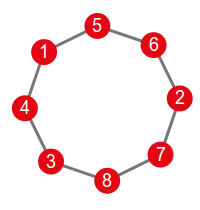
\includegraphics[scale=0.8]{imagenes/faimilia2.png}
\end{center}
  \caption{Circuito simple rotulado ``en orden''}\label{fig:familia2}
\endminipage\hfill
\minipage{0.5\textwidth}
\begin{center}
  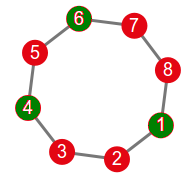
\includegraphics[scale=0.8]{imagenes/faimilia2-resopt.png}
\end{center}
  \caption{Solución hallada por nuestra heurística}\label{fig:familia2res}
\endminipage\\
\minipage{0.5\textwidth}
\begin{center}
  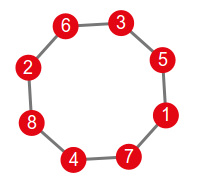
\includegraphics[scale=1.0]{imagenes/faimilia2rename.png}
\end{center}
  \caption{Circuito simple rotulado ``no en orden''}\label{fig:familia2bis}
\endminipage\hfill
\minipage{0.5\textwidth}
\begin{center}
  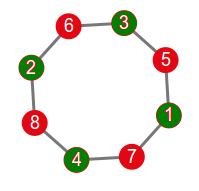
\includegraphics[scale=1.0]{imagenes/faimilia2rename-solnoopt.png}
\end{center}
  \caption{Solución hallada por nuestra heurística}\label{fig:familia2bisres}
\endminipage
\end{figure}



\vspace*{0.6cm}

\subsection{Instancias óptimas.}

\vspace*{0.3cm}

A continuación presentaremos una familia de grafos para la cual nuestra heurística golosa siempre encuentra una solución óptima.

La forma de los grafos pertenecientes a esta familia responde a las siguientes características:

\begin{itemize}
\item Existe un único vértice $v$ que llamaremos ``central'', con grado $\delta(v)$.
\item Para cada vértice $w$ adyacente a $v$, $\delta(w) > \delta(v)$, y sus nodos adyacentes (salvo $v$) tienen grado 1.	
\end{itemize}

Dado que el algoritmo propuesto va tomando en cada paso el nodo ``óptimo'', o sea, aquél que más nodos ``libres'' cubre, en un grafo como el descrito se irá formando el conjunto solución con los vértices adyacentes al nodo ``central'' $v$.  

FALTA MOSTRAR QUE ES LA MEJOR

La Figura \ref{fig:familia3} muestra un ejemplo de grafo perteneciente a esta familia, y la Figura \ref{fig:familia3res} muestra en color verde la solución hallada por nuestro algoritmo.

\begin{figure}[!htb]
\minipage{0.5\textwidth}
\begin{center}
  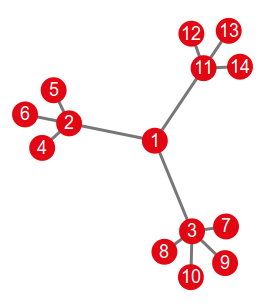
\includegraphics[scale=0.5]{imagenes/familia3.png}
\end{center}
  \caption{Grafo perteneciente a la Familia óptima}\label{fig:familia3}
\endminipage\hfill
\minipage{0.5\textwidth}
\begin{center}
  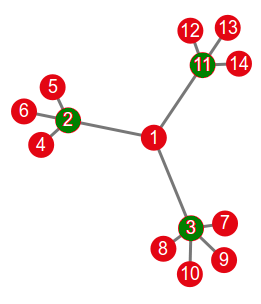
\includegraphics[scale=0.5]{imagenes/familia3-res.png}
\end{center}
  \caption{Solución hallada por nuestra heurística}\label{fig:familia3res}
\endminipage
\end{figure}


\vspace*{0.6cm}

\subsection{Experimentación y gráficos.}

\vspace*{0.3cm}

\vspace*{0.6cm}

\subsubsection{Test 1}
\vspace*{0.3cm}

\vspace*{0.6cm}
%\newpage

\subsubsection{Test 2}

